%package list
\documentclass{article}
\usepackage[top=3cm, bottom=3cm, outer=3cm, inner=3cm]{geometry}
\usepackage{multicol}
\usepackage{graphicx}
\usepackage{url}
%\usepackage{cite}
\usepackage{hyperref}
\usepackage{array}
%\usepackage{multicol}
\newcolumntype{x}[1]{>{\centering\arraybackslash\hspace{0pt}}p{#1}}
\usepackage{natbib}
\usepackage{pdfpages}
\usepackage{multirow}
\usepackage[normalem]{ulem}
\useunder{\uline}{\ul}{}
\usepackage{svg}
\usepackage{xcolor}
\usepackage{listings}
\lstdefinestyle{ascii-tree}{
    literate={├}{|}1 {─}{--}1 {└}{+}1 
  }
\lstset{basicstyle=\ttfamily,
  showstringspaces=false,
  commentstyle=\color{red},
  keywordstyle=\color{blue}
}
%\usepackage{booktabs}
\usepackage{caption}
\usepackage{subcaption}
\usepackage{float}
\usepackage{array}

\newcolumntype{M}[1]{>{\centering\arraybackslash}m{#1}}
\newcolumntype{N}{@{}m{0pt}@{}}


%%%%%%%%%%%%%%%%%%%%%%%%%%%%%%%%%%%%%%%%%%%%%%%%%%%%%%%%%%%%%%%%%%%%%%%%%%%%
%%%%%%%%%%%%%%%%%%%%%%%%%%%%%%%%%%%%%%%%%%%%%%%%%%%%%%%%%%%%%%%%%%%%%%%%%%%%
\newcommand{\itemEmail}{schirinosne@unsa.edu.pe}
\newcommand{\itemStudent}{Sebastian Arley Chirinos Negrón}
\newcommand{\itemCourse}{Estructura de datos y Algoritmos}
\newcommand{\itemCourseCode}{1702124}
\newcommand{\itemSemester}{I}
\newcommand{\itemUniversity}{Universidad Nacional de San Agustín de Arequipa}
\newcommand{\itemFaculty}{Facultad de Ingeniería de Producción y Servicios}
\newcommand{\itemDepartment}{Departamento Académico de Ingeniería de Sistemas e Informática}
\newcommand{\itemSchool}{Escuela Profesional de Ingeniería de Sistemas}
\newcommand{\itemAcademic}{2023 - A}
\newcommand{\itemInput}{17 Junio 2023}
\newcommand{\itemOutput}{23 Julio 2023}
\newcommand{\itemPracticeNumber}{07}
\newcommand{\itemTheme}{Tries}
%%%%%%%%%%%%%%%%%%%%%%%%%%%%%%%%%%%%%%%%%%%%%%%%%%%%%%%%%%%%%%%%%%%%%%%%%%%%
%%%%%%%%%%%%%%%%%%%%%%%%%%%%%%%%%%%%%%%%%%%%%%%%%%%%%%%%%%%%%%%%%%%%%%%%%%%%

\usepackage[english,spanish]{babel}
\usepackage[utf8]{inputenc}
\AtBeginDocument{\selectlanguage{spanish}}
\renewcommand{\figurename}{Figura}
\renewcommand{\refname}{Referencias}
\renewcommand{\tablename}{Tabla} %esto no funciona cuando se usa babel
\AtBeginDocument{%
	\renewcommand\tablename{Tabla}
}

\usepackage{fancyhdr}
\pagestyle{fancy}
\fancyhf{}
\setlength{\headheight}{30pt}
\renewcommand{\headrulewidth}{1pt}
\renewcommand{\footrulewidth}{1pt}
\fancyhead[L]{\raisebox{-0.2\height}{
\includegraphics[width=3cm]{img/logo_episunsa.png}}}
\fancyhead[C]{\fontsize{7}{7}\selectfont	\itemUniversity \\ \itemFaculty \\ \itemDepartment \\ \itemSchool \\ \textbf{\itemCourse}}
\fancyhead[R]{\raisebox{-0.2\height}{
\includegraphics[width=1.2cm]{img/logo_abet}}}
\fancyfoot[L]{Sebastian Chirinos Negrón}
\fancyfoot[C]{\itemCourse}
\fancyfoot[R]{Página \thepage}

% para el codigo fuente
\usepackage{listings}
\usepackage{color, colortbl}
\definecolor{dkgreen}{rgb}{0,0.6,0}
\definecolor{gray}{rgb}{0.5,0.5,0.5}
\definecolor{mauve}{rgb}{0.58,0,0.82}
\definecolor{codebackground}{rgb}{72, 0.95, 0.92}
\definecolor{tablebackground}{rgb}{0.8, 0, 0}

\lstset{frame=tb,
	language=bash,
	aboveskip=3mm,
	belowskip=3mm,
	showstringspaces=false,
	columns=flexible,
	basicstyle={\small\ttfamily},
	numbers=none,
	numberstyle=\tiny\color{gray},
	keywordstyle=\color{blue},
	commentstyle=\color{dkgreen},
	stringstyle=\color{mauve},
	breaklines=true,
	breakatwhitespace=true,
	tabsize=3,
	backgroundcolor= \color{codebackground},
}

\begin{document}
	
	\vspace*{10px}
	
	\begin{center}	
		\fontsize{17}{17} \textbf{ Informe de Laboratorio \itemPracticeNumber}
	\end{center}
	\centerline{\textbf{\Large Tema: \itemTheme}}
	%\vspace*{0.5cm}	

	\begin{flushright}
		\begin{tabular}{|M{2.5cm}|N|}
			\hline 
			\rowcolor{tablebackground}
			\color{white} \textbf{Nota}  \\
			\hline 
			     \\[30pt]
			\hline 			
		\end{tabular}
	\end{flushright}	

	\begin{table}[H]
		\begin{tabular}{|x{4.7cm}|x{4.8cm}|x{4.8cm}|}
			\hline 
			\rowcolor{tablebackground}
			\color{white} \textbf{Estudiante} & \color{white}\textbf{Escuela}  & \color{white}\textbf{Asignatura}   \\
			\hline 
			{\itemStudent \par \itemEmail} & \itemSchool & {\itemCourse \par Semestre: \itemSemester \par Código: \itemCourseCode}     \\
			\hline 			
		\end{tabular}
	\end{table}		
	
	\begin{table}[H]
		\begin{tabular}{|x{4.7cm}|x{4.8cm}|x{4.8cm}|}
			\hline 
			\rowcolor{tablebackground}
			\color{white}\textbf{Laboratorio} & \color{white}\textbf{Tema}  & \color{white}\textbf{Duración}   \\
			\hline 
			\itemPracticeNumber & \itemTheme & 04 horas   \\
			\hline 
		\end{tabular}
	\end{table}
	
	\begin{table}[H]
		\begin{tabular}{|x{4.7cm}|x{4.8cm}|x{4.8cm}|}
			\hline 
			\rowcolor{tablebackground}
			\color{white}\textbf{Semestre académico} & \color{white}\textbf{Fecha de inicio}  & \color{white}\textbf{Fecha de entrega}   \\
			\hline 
			\itemAcademic & \itemInput &  \itemOutput  \\
			\hline 
		\end{tabular}
	\end{table}
	
	\section{Tarea}
	\subsection{Trie}
	\begin{itemize}
		
	\item Trie es un tipo de árbol de búsqueda k-ario utilizado para almacenar y buscar una clave específica de un conjunto.

	\item Con Trie, las complejidades de búsqueda se pueden llevar al límite óptimo (longitud de clave).

	\item Un trie (derivado de recuperación) es una estructura de datos de árbol de varias vías que se utiliza para almacenar cadenas en un alfabeto.

	\item Se utiliza para almacenar una gran cantidad de cadenas. La coincidencia de patrones se puede hacer de manera eficiente usando intentos.

	\end{itemize}	
		

	\section{URL de Repositorio Github}
	\begin{itemize}
		\item URL del Repositorio GitHub para clonar o recuperar.
		\item \url{https://github.com/BastleyNait/EDA-LAB-B-23A.git}
		\item URL para el laboratorio 07 en el Repositorio GitHub.
		\item \url{https://github.com/BastleyNait/EDA-LAB-B-23A/tree/main/lab07}
	\end{itemize}
	
	\section{Ejercicios designados}

	\subsection{Clase NodeTrie}
	\begin{itemize}
		\item Línea 1: Se importa la clase Arrays del paquete java.util, que proporciona métodos para trabajar con matrices (arrays).

	\item Línea 3: Se define una clase llamada NodeTrie que utiliza un tipo genérico T para representar el tipo de datos almacenado en los nodos del Trie.

	\item Línea 9: Se declara una variable booleana isEndOfWord que indica si el nodo actual representa el final de una palabra en el Trie.

	\item Línea 10: Se define un método getter getRepeticiones() que devuelve el arreglo de repeticiones.

	\item Línea 14: Se define un método setter setRepeticiones() que establece el arreglo de repeticiones con un nuevo valor.

	\item Línea 16: Se crea el constructor de la clase NodeTrie, que inicializa la variable isEndOfWord en false y rellena el arreglo children con valores nulos utilizando Arrays.fill().

	\item Línea 22: Se define un método getter getChildren() que devuelve el arreglo de nodos hijos del nodo actual.

	\item Línea 26: Se define un método setter setChildren() que establece el arreglo de nodos hijos del nodo actual con un nuevo arreglo.

	\item Línea 30: Se define un método getter isEndOfWord() que devuelve el valor de la variable isEndOfWord, indicando si el nodo representa el final de una palabra.

	\item Línea 34: Se define un método setter setEndOfWord() que establece el valor de la variable isEndOfWord, indicando si el nodo representa el final de una palabra.
	\end{itemize}

	\lstinputlisting[language=Java, caption={NodeTrie.java},numbers=left,]{src/NodeTrie.java}	

	

	%%%%%%%%%%%%%%%%%%%%%%%%%%%%%%%%%%%%%%%%%%%%%%%%%%%%%%%%%%%%%%%%%%%%%%%%%%%%%%%%%%%%%%%%%%%%%
	\subsection{Clase Trie}
	\begin{itemize}	
		\item \textbf{public class Trie<T>:} Se define una clase llamada Trie que utiliza un tipo genérico T para representar el tipo de datos almacenado en el Trie.

		\item \textbf{private NodeTrie<T> root = new NodeTrie<>();}: Se declara y se inicializa la raíz del Trie como un nuevo nodo Trie utilizando el tipo genérico T.

		\item \textbf{private int contPala = 0;}: Se declara una variable contPala para contar el número total de palabras almacenadas en el Trie.

		\item \textbf{public boolean insert(String key):} Se define un método público llamado insert que recibe una cadena key como parámetro y retorna un booleano. Este método se utiliza para insertar una palabra en el Trie.

		\item \textbf{NodeTrie<T> aux = this.root;}: Se declara una variable aux y se inicializa con la raíz del Trie. Esta variable se utiliza para recorrer el Trie durante la inserción.

		\item \textbf{Líneas 10-15:} Se realiza un bucle para recorrer cada carácter de la palabra key y se verifica si es una letra del alfabeto (entre 'a' y 'z') o la letra "ñ" (representada por el carácter 164). Si el carácter es válido, se avanza al siguiente nodo Trie correspondiente al carácter actual.

		\item \textbf{Línea 18:} Se comprueba si el último carácter de la palabra key es una letra válida del alfabeto o la letra "ñ". Si es válido, se realiza la inserción de la palabra en el Trie.

		\item \textbf{Línea 19-22:} Si el nodo actual es el final de una palabra (isEndOfWord es verdadero), se incrementa el contador de repeticiones para el carácter actual. Si no, se marca el nodo actual como el final de una palabra, se incrementa el contador de repeticiones para el carácter actual y se incrementa el contador total de palabras contPala.

		\item \textbf{public boolean delete(String key):} Se define un método público llamado delete que recibe una cadena key como parámetro y retorna un booleano. Este método se utiliza para eliminar una palabra del Trie.

		\item \textbf{Líneas 37-43:} Se realiza un bucle similar al del método insert para recorrer cada carácter de la palabra key. Si el carácter es válido y el nodo correspondiente no es nulo, se elimina el enlace entre el nodo actual y el siguiente nodo correspondiente al carácter actual.

		\item \textbf{Línea 46-49:} Se realiza una comprobación similar al método insert para marcar el nodo final de la palabra como falso (es decir, no es el final de una palabra), se incrementa el contador de repeticiones para el carácter actual y se decrementa el contador total de palabras contPala.

		\item \textbf{public int search(String key):} Se define un método público llamado search que recibe una cadena key como parámetro y retorna un entero. Este método se utiliza para buscar una palabra en el Trie y devuelve el número de repeticiones de la palabra encontrada.

		\item \textbf{Línea 51:} Se declara una variable aux y se inicializa con la raíz del Trie. Esta variable se utiliza para recorrer el Trie durante la búsqueda.

		\item \textbf{Línea 52:} Se declara una variable cont para almacenar el número de repeticiones de la palabra encontrada y se inicializa en 0.

		\item \textbf{Líneas 55-60:} Se realiza un bucle para recorrer cada carácter de la palabra key. Si el carácter es válido y el nodo correspondiente no es nulo, se avanza al siguiente nodo correspondiente al carácter actual. Si se encuentra el final de la palabra (isEndOfWord es verdadero) en algún punto del recorrido, se obtiene el número de repeticiones para el carácter actual y se asigna a la variable cont.

		\item \textbf{Línea 65:} Se devuelve el valor de cont, que representa el número de repeticiones de la palabra encontrada, o 0 si la palabra no se encuentra en el Trie.

		\item \textbf{public int numDePalabras():} Se define un método público llamado numDePalabras que no recibe parámetros y retorna un entero. Este método se utiliza para obtener el número total de palabras almacenadas en el Trie.

		\item \textbf{Línea 67:} Se devuelve el valor de la variable contPala, que representa el número total de palabras almacenadas en el Trie.
	\end{itemize}	
	
	\lstinputlisting[language=Java, caption={Trie.java},numbers=left,]{src/Trie.java}	

%%%%%%%%%%%%%%%%%%%%%%%%%%%%%%%%%%%%%%%%%%%%%%%%%%%%%%%%%%%%%%%%%%%%%%%%%%%%%%%%%%%%%%%%%%%%%%%%%%%%%%%%%%
\subsection{Clase TextMod.java}
\begin{itemize}	
	\item En resumen, este código define una clase TexMod que representa una aplicación de editor de texto con una GUI. Utiliza una estructura de datos Trie para almacenar y buscar palabras en el texto de manera eficiente. La aplicación permite realizar operaciones como buscar, eliminar y reemplazar palabras en el texto, y muestra los resultados en una interfaz gráfica personalizada con el tema FlatMacDarkLaf.
\end{itemize}	
\lstinputlisting[language=Java, caption={TextMod.java},numbers=left,]{src/TextMod.java}	
\begin{itemize}
	\item \textbf{import com.formdev.flatlaf.themes.FlatMacDarkLaf;}: Se importa la clase FlatMacDarkLaf del paquete com.formdev.flatlaf.themes, que es utilizada para personalizar el tema de la GUI en un estilo oscuro similar al tema de macOS.

		\item \textbf{import javax.swing.*;}: Se importa el paquete javax.swing.*, que contiene clases y componentes para la creación de interfaces gráficas.

		\item \textbf{import java.awt.event.ActionEvent;}: Se importa el paquete java.awt.event.ActionEvent, que contiene la clase ActionEvent, utilizada para representar eventos de acción.

		\item \textbf{private JPanel mainPanel;}: Se declara una variable de instancia llamada mainPanel, que representa un panel principal en la interfaz.

		\item \textbf{Líneas 8 a 19:} Se declaran diversas variables de instancia que representan los componentes de la interfaz gráfica, tales como campos de texto, botones y áreas de texto.

		\item \textbf{private Trie<Character> miTrie = new Trie<>();}: Se declara una variable de instancia llamada miTrie, que es una estructura de datos Trie utilizada para almacenar y buscar palabras eficientemente. Se especifica que la clave del Trie será de tipo Character.

		\item {public TexTool() {:} Se define el constructor de la clase TexTool, que se ejecutará cuando se cree un objeto de esta clase.

		\item \textbf{Líneas 14 a 29:} En el constructor, se configura el contenido principal y algunas propiedades de la ventana. Se agregan ActionListener a los botones para manejar eventos de clic.

		\item {public static void main(String[] args) {:} Se define el método main, que es el punto de entrada del programa.

		\item {Líneas 33 a 36:} En el método main, se configura el tema FlatMacDarkLaf para personalizar la apariencia de la interfaz gráfica.

		\item {public String insertar(String texto) {:} Se define el método insertar, que recibe un texto como parámetro y lo divide en palabras para insertarlas en el Trie.

		\item {Líneas 39 a 47:} En el método insertar, se divide el texto en palabras y se inserta cada palabra en el Trie, teniendo en cuenta los signos de puntuación al final de las palabras.

		\item {public String eliminar(String palabra, String[] texto) {:} Se define el método eliminar, que recibe una palabra y un arreglo de texto, y elimina la palabra del texto.

		\item {Líneas 50 a 60:} En el método eliminar, se realiza la eliminación de la palabra del texto y se obtiene el texto resultante.

		\item {public String reemplazar(String palabra, String newPalabra, String[] texto) {:} Se define el método reemplazar, que recibe una palabra, una nueva palabra y un arreglo de texto, y realiza el reemplazo de la palabra en el texto.

		\item {Líneas 63 a 73:} En el método reemplazar, se realiza el reemplazo de la palabra en el texto y se obtiene el texto resultante.

		\item {public String buscar(String palabra, String[] texto) {:} Se define el método buscar, que recibe una palabra y un arreglo de texto, y busca la palabra en el texto resaltándola.

		\item \textbf{Líneas 76 a 86:} En el método buscar, se realiza la búsqueda de la palabra en el texto y se obtiene el texto resultante con la palabra resaltada en un fondo de color.
\end{itemize}

%%%%%%%%%%%%%%%%%%%%%%%%%%%%%%%%%%%%%%%%%%%%%%%%%%%%%%%%%%%%%%%%%%%%%%%%%%%%%%%%%%%%%%%%%%%%%%%%%%
\subsection{GUI TextMod.form}
\begin{itemize}	
	\item archivo XML que define la estructura y disposición de componentes de una interfaz gráfica de usuario (GUI) para una aplicación llamada "TexT MoD". La GUI está diseñada para un editor de texto con funcionalidades de búsqueda, reemplazo y eliminación de palabras en un texto.

\end{itemize}	
\lstinputlisting[language=Java, caption={TextMod.form},numbers=left,]{src/TextMod.form}	
\begin{itemize}
	\item \textbf{Línea 1:} Declaración de la versión y codificación del archivo XML.

	\item \textbf{Línea 2 a 38:} Definición de la estructura de la GUI utilizando etiquetas XML. La GUI se compone principalmente de un panel principal ("mainPanel") con diferentes componentes, como etiquetas ("javax.swing.JLabel"), campos de texto ("javax.swing.JTextField"), área de texto ("javax.swing.JTextArea"), editor de texto ("javax.swing.JEditorPane") y botones ("javax.swing.JButton").

	\item \textbf{Línea 7 a 10:} Se establecen las propiedades y restricciones para el panel principal.

	\item \textbf{Línea 11 a 13:} Se establecen las propiedades y restricciones para una etiqueta que muestra el título de la aplicación ("TexT MoD").

	\item \textbf{Línea 15 a 30:} Se definen componentes para ingresar texto ("Ingrese su texto:"), y una área de texto donde se mostrará el texto ingresado ("Texto").

	\item \textbf{Línea 32 a 35:} Se definen componentes para ingresar una palabra a buscar ("Buscar:") y el resultado de la búsqueda ("Resultado:").

	\item \textbf{Línea 37 a 53:} Se definen componentes para ingresar una palabra a eliminar ("Eliminar:") y botones para realizar las acciones de buscar, eliminar y reemplazar palabras en el texto.
\end{itemize}
\subsection{Ejecución}
\begin{itemize}	
	\item BUSQUEDA
\end{itemize}	
\begin{figure}[H]
	\centering
	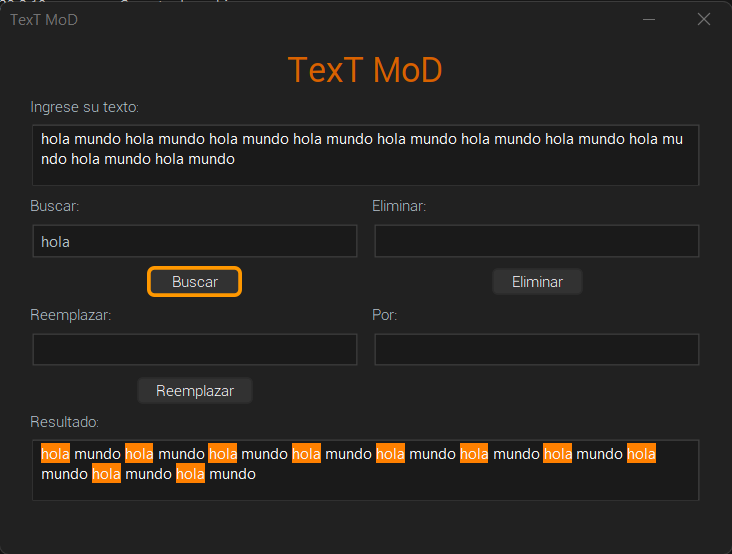
\includegraphics[width=0.7\textwidth,keepaspectratio]{img/busqueda.png}
	%\includesvg{img/automata.svg}
	%\label{img:mot2}
	%\caption{Product backlog.}
\end{figure}
\begin{itemize}	
	\item ELIMINACION
\end{itemize}	

\begin{figure}[H]
	\centering
	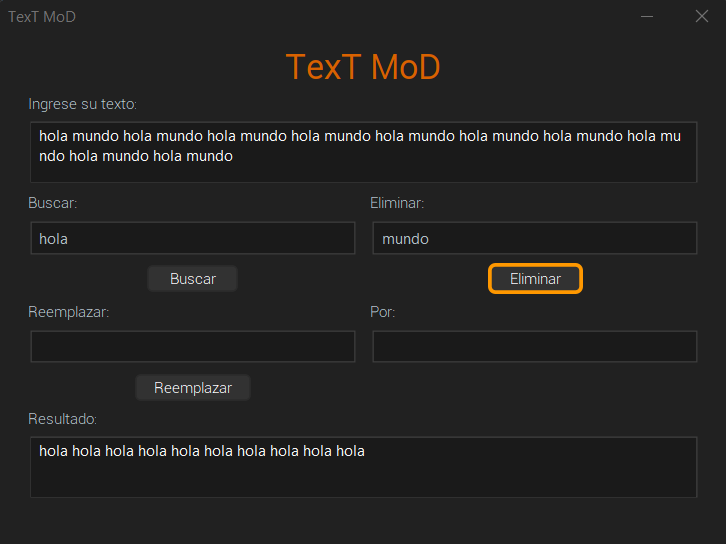
\includegraphics[width=0.7\textwidth,keepaspectratio]{img/eliminacion.png}
	%\includesvg{img/automata.svg}
	%\label{img:mot2}
	%\caption{Product backlog.}
\end{figure}
\begin{itemize}	
	\item REMPLAZO
\end{itemize}	

\begin{figure}[H]
	\centering
	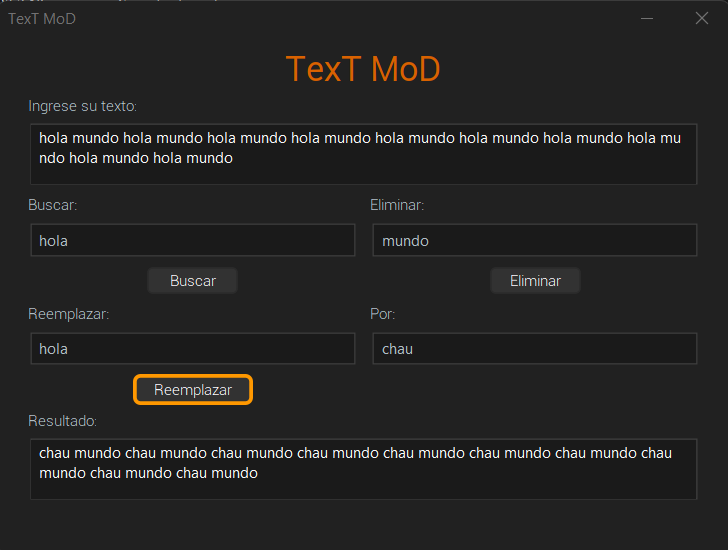
\includegraphics[width=0.7\textwidth,keepaspectratio]{img/remplazo.png}
	%\includesvg{img/automata.svg}
	%\label{img:mot2}
	%\caption{Product backlog.}
\end{figure}

%%%%%%%%%%%%%%%%%%%%%%%%%%%%%%%%%%%%%%%%%%%%%%%%%%%%%%%%%%%%%%%%%%%%%%%%%%%%%%%%%%


	\subsection{Commits del trabajo}
	\begin{itemize}	
		\item Acá estan algunos de los commits mas importantes en este trabajo:
	\end{itemize}	
	
	\begin{figure}[H]
		\centering
		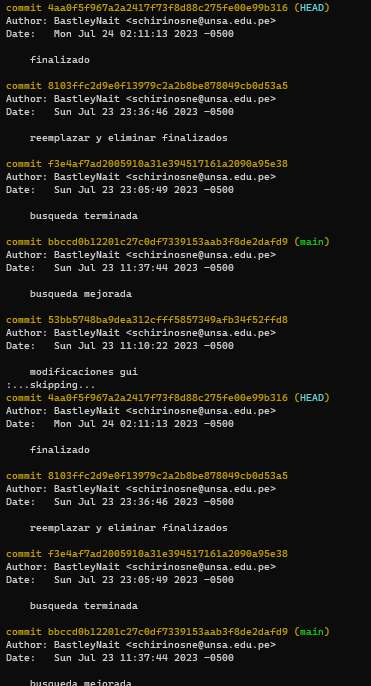
\includegraphics[width=0.7\textwidth,keepaspectratio]{img/Commits.png}
		%\includesvg{img/automata.svg}
		%\label{img:mot2}
		%\caption{Product backlog.}
	\end{figure}


%%%%%%%%%%%%%%%%%%%%%%%%%%%%%%%%%%%%%%%%%%%%%%%%%%%%%%%%%%%%%%%%%%%%%%%%%%%%%%%%%%
\subsection{Instrucciones para la ejecucion}
\begin{itemize}	
	\item Se adjunto en el repositorio un archivo ejecutable \textbf{App.jar} para que pueda ser testeado desde cualquier pc
	\item Se hizo con ejecutable ya que intellij idea tiene muchas dependencias para que pueda funcionar correctamente java swing
	\item por lo que es una tarea un tanto compleja, para ello se creo el archivo \textbf{App.jar}
\end{itemize}	
		
	\subsection{Estructura de laboratorio 07}
	\begin{itemize}	
		\item El contenido que se entrega en este laboratorio es el siguiente:
	\end{itemize}
	
\begin{lstlisting}[style=ascii-tree]
lab06/
|   .gitignore
|	Trie.java
|	TextMod.java
|	TextMod.form
|	NodeTrie.java

\---latex
    |	EDA_lab07_schirinosne.pdf
    |   EDA_lab07_schirinosne.tex
    |
    +---img
    |       Commits.png
    |       logo_abet.png
    |       logo_episunsa.png
    |       logo_unsa.jpg
    |       busqueda.jpg  
    |       remplazo.jpg    
    |		eliminacion.jpg
    \---src
			|	Trie.java
			|	TextMod.java
			|	TextMod.form
			|	NodeTrie.java
\end{lstlisting}    


	\section{\textcolor{red}{Rúbricas}}
	
	\subsection{\textcolor{red}{Entregable Informe}}
	\begin{table}[H]
		\caption{Tipo de Informe}
		\setlength{\tabcolsep}{0.5em} % for the horizontal padding
		{\renewcommand{\arraystretch}{1.5}% for the vertical padding
		
		\begin{tabular}{|p{3cm}|p{12cm}|}
			\hline
			\multicolumn{2}{|c|}{\textbf{\textcolor{red}{Informe}}}  \\
			\hline 
			\textbf{\textcolor{red}{Latex}} & \textcolor{blue}{El informe está en formato PDF desde Latex,  con un formato limpio (buena presentación) y facil de leer.}   \\ 
			\hline 
			
			
		\end{tabular}
	}
	\end{table}
	\subsection{\textcolor{red}{Rúbrica para el contenido del Informe y demostración}}
	\begin{itemize}			
		\item El alumno debe marcar o dejar en blanco en celdas de la columna \textbf{Checklist} si cumplio con el ítem correspondiente.
		\item Si un alumno supera la fecha de entrega,  su calificación será sobre la nota mínima aprobada, siempre y cuando cumpla con todos lo items.
		\item El alumno debe autocalificarse en la columna \textbf{Estudiante} de acuerdo a la siguiente tabla:
	
		\begin{table}[ht]
			\caption{Niveles de desempeño}
			\begin{center}
			\begin{tabular}{ccccc}
    			\hline
    			 & \multicolumn{4}{c}{Nivel}\\
    			\cline{1-5}
    			\textbf{Puntos} & Insatisfactorio 25\%& En Proceso 50\% & Satisfactorio 75\% & Sobresaliente 100\%\\
    			\textbf{2.0}&0.5&1.0&1.5&2.0\\
    			\textbf{4.0}&1.0&2.0&3.0&4.0\\
    		\hline
			\end{tabular}
		\end{center}
	\end{table}	
	
	\end{itemize}
	
	\begin{table}[H]
		\caption{Rúbrica para contenido del Informe y demostración}
		\setlength{\tabcolsep}{0.5em} % for the horizontal padding
		{\renewcommand{\arraystretch}{1.5}% for the vertical padding
		%\begin{center}
		\begin{tabular}{|p{2.7cm}|p{7cm}|x{1.3cm}|p{1.2cm}|p{1.5cm}|p{1.1cm}|}
			\hline
    		\multicolumn{2}{|c|}{Contenido y demostración} & Puntos & Checklist & Estudiante & Profesor\\
			\hline
			\textbf{1. GitHub} & Hay enlace URL activo del directorio para el  laboratorio hacia su repositorio GitHub con código fuente terminado y fácil de revisar. &2 &X &2 & \\ 
			\hline
			\textbf{2. Commits} &  Hay capturas de pantalla de los commits más importantes con sus explicaciones detalladas. (El profesor puede preguntar para refrendar calificación). &4 & x&4 & \\ 
			\hline 
			\textbf{3. Código fuente} &  Hay porciones de código fuente importantes con numeración y explicaciones detalladas de sus funciones. &2 &X &2 & \\ 
			\hline 
			\textbf{4. Ejecución} & Se incluyen ejecuciones/pruebas del código fuente  explicadas gradualmente. &2 &X &2 & \\ 
			\hline			
			\textbf{5. Pregunta} & Se responde con completitud a la pregunta formulada en la tarea.  (El profesor puede preguntar para refrendar calificación).  &2 &X &2 & \\ 
			\hline	
			\textbf{6. Fechas} & Las fechas de modificación del código fuente estan dentro de los plazos de fecha de entrega establecidos. &2 &X &2 & \\ 
			\hline 
			\textbf{7. Ortografía} & El documento no muestra errores ortográficos. &2 &X &2 & \\ 
			\hline 
			\textbf{8. Madurez} & El Informe muestra de manera general una evolución de la madurez del código fuente,  explicaciones puntuales pero precisas y un acabado impecable.   (El profesor puede preguntar para refrendar calificación).  &4 &x &4 & \\ 
			\hline
			\multicolumn{2}{|c|}{\textbf{Total}} &20 & &20 & \\ 
			\hline
		\end{tabular}
		%\end{center}
		%\label{tab:multicol}
		}
	\end{table}
	
\clearpage		
\section{Referencias}
\begin{itemize}			
	\item \url{https://www.geeksforgeeks.org/introduction-to-avl-tree/}
	\item \url{https://www.geeksforgeeks.org/insertion-in-an-avl-tree/}
	\item \url{https://www.geeksforgeeks.org/deletion-in-an-avl-tree/}
	\item \url{https://docs.oracle.com/javase/tutorial/java/generics/types.html}
	\item \url{https://algorithmtutor.com/Data-Structures/Tree/AVL-Trees/}

\end{itemize}	

	
%\clearpage
%\bibliographystyle{apalike}
%\bibliographystyle{IEEEtranN}
%\bibliography{bibliography}
			
\end{document}